\documentclass[11pt]{article}

\usepackage{amsmath,amssymb,amsfonts}
\usepackage{geometry}
\usepackage{graphicx}
\usepackage{physics}
\usepackage{bm}
\usepackage{hyperref}
\usepackage{multicol}
\usepackage{caption}
\usepackage{tikz}
\usetikzlibrary{positioning,arrows.meta,calc}

\geometry{margin=1in}

% -----------------------------------------------------------
% Handy macros
% -----------------------------------------------------------
\newcommand{\KL}{D_{\mathrm{KL}}}
\newcommand{\E}{\mathbb{E}}
\newcommand{\mcF}{\mathcal{F}}
\newcommand{\mcS}{\mathcal{S}}

\title{\textbf{Coherence-Driven Active Inference of the Substrate}\\[4pt]
\large{Unified Free-Energy Functional Free-Energy Principle}}
\author{Julien Steff}
\date{}

\begin{document}
\maketitle

\begin{abstract}
This work develops a unified theoretical framework in which the Time-Crystalline Quantum Substrate and Karl Friston's Free-Energy Principle appear as two manifestations of a single free-energy functional defined on an underlying Substrate \(S\). The TCQS picture treats reality as a coherence-driven, Floquet-updated informational substrate, whose dynamics follow a free-energy gradient defined by a coherence potential. Friston's FEP describes biological agents as systems that minimize a variational free energy that upper-bounds sensory surprise under a generative model. Here we: (i) formalize the Substrate \(S\) and a coherence scalar \(C(S)\); (ii) review the variational free energy used in FEP; (iii) derive a unified functional
\[
\boxed{\mcF_{S}[S,q] = \Phi\!\big[C(S)\big] + \KL\big(q(\vartheta|\mu)\,\|\,p(\vartheta|S)\big)}
\]
that couples the coherence potential \(\Phi\) of the substrate with the variational term of FEP; and (iv) show how biological agents arise as coherent submanifolds of \(S\) performing active inference inside the same global free-energy landscape.
\end{abstract}

% =============================================================
% SECTION I — FUNDAMENTAL ONTOLOGY
% =============================================================

\section{The Substrate \(S\) as }

In the TCQS framework, reality is grounded in a Substrate \(S\) that encodes the total informational configuration of the universe. We denote by
\[
S \in \mcS
\]
a point in the configuration space \(\mcS\) of possible global substrate states. Each \(S\) specifies, in principle, all microscopic relations of coherence, phase, and entanglement that underlie the emergent phenomena of fields, particles, and classical spacetime.

The distinctive TCQS move is to treat \(S\) as a \emph{time-crystalline} object: there exists an intrinsic discrete update map
\begin{equation}
U:\mcS \rightarrow \mcS, \qquad S_{n+1} = U(S_n)
\end{equation}
with Floquet-like periodicity and self-referential structure. The continuous-time limit can be written as a flow
\begin{equation}
\dot{S}(t) = F\big(S(t)\big),
\end{equation}
where the vector field \(F\) is determined by informational coherence constraints rather than purely local differential equations on a pre-given spacetime.

\subsection{Coherence Scalar on the Substrate}

We assume the existence of a \emph{coherence functional}
\begin{equation}
C:\mcS \rightarrow \mathbb{R},
\end{equation}
assigning to each global substrate state \(S\) a scalar measure of its informational coherence (or equivalently, inverse decoherence / disorder). High \(C(S)\) corresponds to states in which quasi-classical structures (stable waves, particles, atoms, and organisms) are supported by deep, resonant patterns of the substrate.

The TCQS picture then introduces a \emph{coherence potential} \(\Phi\) acting on this scalar:
\begin{equation}
\Phi:\mathbb{R} \rightarrow \mathbb{R}, \qquad \Phi = \Phi\big(C(S)\big).
\end{equation}
We will only require that \(\Phi\) is monotonically decreasing in \(C\): higher coherence lowers the potential.

\subsection{Substrate-Level Free-Energy Gradient}

The simplest dynamical ansatz consistent with the TCQS intuition is that the substrate flows down the gradient of \(\Phi\):
\begin{equation}
\dot{S}(t) = -\,\nabla_{S}\,\Phi\!\big(C(S)\big).
\label{eq:substrate-flow}
\end{equation}
Here \(\nabla_{S}\) is defined with respect to an appropriate metric on configuration space. Equation \eqref{eq:substrate-flow} is the TCQS analogue of a free-energy gradient flow: reality moves along trajectories that increase coherence and reduce the coherence potential.

In this sense, \(\Phi\) plays the role of a \emph{global free energy} of the substrate, purely at the level of informational geometry, independent of any particular biological agent.

\section{Friston's Free-Energy Principle in Brief}

Friston's Free-Energy Principle (FEP) addresses a different level of description: the behaviour of \emph{adaptive, self-organizing subsystems} such as brains and organisms. Let us recall the core elements.

\subsection{Generative Model and Recognition Density}

Consider an agent that samples sensory data \(s\) from the environment. The agent entertains a generative model \(p(s,\vartheta)\), where \(\vartheta\) denotes hidden causes (states, parameters) in the model. Direct Bayesian inference of \(p(\vartheta|s)\) is intractable in general, so the agent represents an approximate posterior or \emph{recognition density} \(q(\vartheta|\mu)\) parameterized by internal states \(\mu\).

\subsection{Variational Free Energy}

The variational free energy associated with a given recognition density is
\begin{equation}
F_{\mathrm{var}}(s,q) 
= \E_{q(\vartheta|\mu)}[-\ln p(s,\vartheta)] 
   - H\big(q(\vartheta|\mu)\big),
\label{eq:F-var-def}
\end{equation}
where \(H\) is the Shannon entropy. This can be re-expressed as
\begin{equation}
F_{\mathrm{var}}(s,q) 
= \KL\!\big(q(\vartheta|\mu)\,\|\,p(\vartheta|s)\big)
  - \ln p(s),
\end{equation}
so that \(F_{\mathrm{var}}\) forms an upper bound on surprise \(-\ln p(s)\). Minimizing \(F_{\mathrm{var}}\) with respect to \(q\) (or equivalently \(\mu\)) makes \(q(\vartheta|\mu)\) approach the true posterior, while minimizing with respect to action modifies the data \(s\) so as to render them more predictable (active inference).

\section{Embedding Agents in the Substrate \(S\)}

To unify TCQS and FEP, we now explicitly regard the environment of an agent as a slice of the substrate \(S\).

\subsection{Agents as Coherent Submanifolds}

Let \(A\subset \mcS\) denote the set of substrate degrees of freedom corresponding to a particular agent (its body, brain, and immediate sensory interface). We denote by \(S_A\) the restriction of the global state \(S\) to those degrees of freedom, and by \(S_{\bar{A}}\) the complement (the rest of the universe).

The key TCQS assumption is that agents are persistent, high-coherence submanifolds:
\begin{equation}
C(S_A) \gg C(S_{\bar{A}}) \quad \text{locally in configuration space.}
\end{equation}
This makes agents robust ``coherence pockets'' embedded in the larger substrate.

\subsection{Sensory States as Functions of \(S\)}

Sensory data \(s\) can now be viewed as functions of the substrate:
\begin{equation}
s = \sigma(S_A,S_{\bar{A}}),
\end{equation}
for some encoding map \(\sigma\) that extracts the agent-relevant boundary conditions from \(S\). In particular, the generative model of the agent can be recast as a model conditioned on the substrate:
\begin{equation}
p(s,\vartheta) \equiv p\big(s,\vartheta \mid S\big),
\end{equation}
and therefore the posterior becomes \(p(\vartheta|s,S)\). When we write \(p(\vartheta|S)\) below, we mean the distribution over latent causes compatible with the substrate state that gives rise to particular sensory patterns for the agent.

\section{Deriving a Unified Free-Energy Functional on \(S\)}

We now derive the unified expression the way you requested: \emph{with the Substrate \(S\) as the fundamental object}.

\subsection{Substrate-Level Potential as a Prior over \(S\)}

Assume that the coherence potential \(\Phi[C(S)]\) induces an effective stationary distribution over substrate configurations:
\begin{equation}
P(S) \propto \exp\big(-\Phi[C(S)]\big).
\label{eq:substrate-gibbs}
\end{equation}
States with high coherence (low \(\Phi\)) are exponentially favoured. This is formally analogous to a Gibbs distribution, but with \(\Phi\) playing the role of generalized free energy rather than thermodynamic energy.

\subsection{Joint Description: Substrate + Agent Beliefs}

The joint description of the universe plus an embedded agent can be written in terms of:
\begin{itemize}
    \item the actual substrate state \(S\),
    \item the agent's internal recognition density \(q(\vartheta|\mu)\) over latent causes.
\end{itemize}
The agent's generative model uses \(p(\vartheta|S)\) as the substrate-conditioned prior over causes.

Given a particular global state \(S\), the mismatch between the agent's beliefs and the substrate-induced distribution over causes is measured by the Kullback--Leibler divergence
\begin{equation}
\KL\big(q(\vartheta|\mu)\,\|\,p(\vartheta|S)\big).
\end{equation}

\subsection{Unified Functional}

We now define the \emph{unified free-energy functional} on the pair \((S,q)\) by
\begin{equation}
\boxed{
\mcF_{S}[S,q] 
= \Phi\!\big[C(S)\big]
+ \KL\!\big(q(\vartheta|\mu)\,\|\,p(\vartheta|S)\big).
}
\label{eq:unified-F}
\end{equation}

This expression has the structure you wanted:

\begin{itemize}
    \item The first term \(\Phi[C(S)]\) is purely substrate-level: it measures how coherent the global configuration is.
    \item The second term is exactly the variational term that appears in Friston-style free energy, but now explicitly conditioned on \(S\).
\end{itemize}

\subsection{Gradient Flows on Substrate and States}

We assume that the dynamics of the universe and the internal states of the agent jointly follow a gradient flow of \(\mcF_{S}\):
\begin{align}
\dot{S} &= -\,\eta_S \,\nabla_{S}\,\mcF_{S}[S,q],
\label{eq:flow-S}\\[4pt]
\dot{\mu} &= -\,\eta_\mu \,\nabla_{\mu}\,\mcF_{S}[S,q],\\[4pt]
\dot{a} &= -\,\eta_a \,\nabla_{a}\,\mcF_{S}[S,q],
\end{align}
where \(a\) denotes the agent's actions and \(\eta_S,\eta_\mu,\eta_a>0\) are step-size parameters.

Using \eqref{eq:unified-F}, the substrate dynamics become
\begin{equation}
\dot{S} = -\,\eta_S \,\nabla_{S}\Phi\!\big[C(S)\big]
          -\,\eta_S\,\nabla_{S}\KL\big(q(\vartheta|\mu)\,\|\,p(\vartheta|S)\big).
\end{equation}
The first term reproduces the TCQS coherence-gradient flow \eqref{eq:substrate-flow}; the second term encodes a subtle back-reaction of agent-level inference on the substrate configuration. In most physical regimes this back-reaction is negligible, but conceptually it closes the loop: agents are not separate from the substrate, they are coherent patterns within it.

Similarly, gradients with respect to \(\mu\) and \(a\) recover the usual FEP dynamics:
\begin{equation}
\dot{\mu},\dot{a} \propto -\nabla_{\mu,a}\,\KL\big(q(\vartheta|\mu)\,\|\,p(\vartheta|S)\big),
\end{equation}
since \(\Phi\) does not depend on \(\mu\) or \(a\). Thus \emph{agents inside \(S\) still perform active inference}, but this is now seen as a local optimization inside a global coherence-driven computation.

\section{Diagram: Mapping FEP \texorpdfstring{$\rightarrow$}{→} TCQS via \(S\)}

The following TikZ diagram is fixed so that the boxes no longer overlap (we use the \texttt{positioning} library and a larger node distance):

\begin{center}
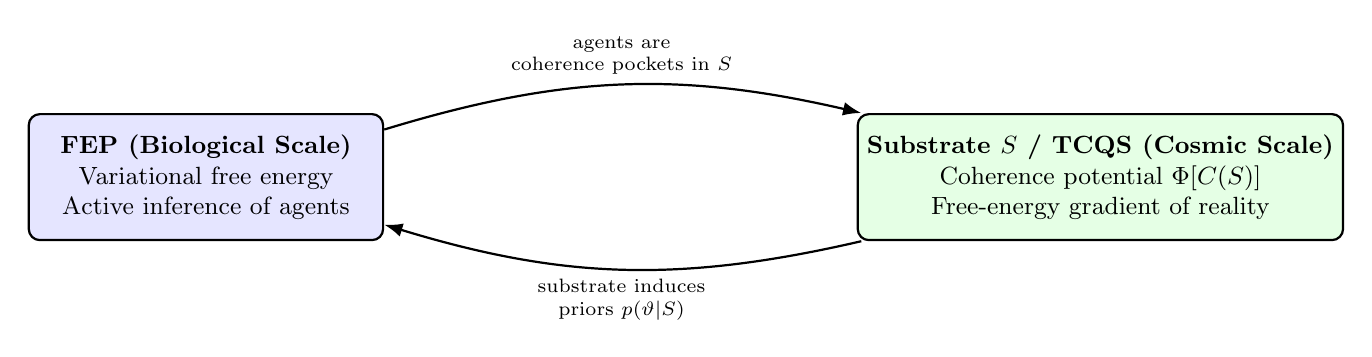
\begin{tikzpicture}[
    node distance=6cm,
    >=Latex,
    thick,
    box/.style={
        rectangle,
        rounded corners,
        draw,
        minimum width=4.5cm,
        minimum height=1.6cm,
        align=center,
        font=\small
    }
]

\node[box, fill=blue!10] (FEP) {
\textbf{FEP (Biological Scale)}\\
Variational free energy\\
Active inference of agents
};

\node[box, fill=green!10, right=of FEP] (TCQS) {
\textbf{Substrate \(S\) / TCQS (Cosmic Scale)}\\
Coherence potential \(\Phi[C(S)]\)\\
Free-energy gradient of reality
};

\draw[->] (FEP) to[bend left=15] node[above,align=center,font=\scriptsize] {agents are\\coherence pockets in \(S\)} (TCQS);
\draw[->] (TCQS) to[bend left=15] node[below,align=center,font=\scriptsize] {substrate induces\\priors \(p(\vartheta|S)\)} (FEP);

\end{tikzpicture}
\end{center}

This visually encodes the two-way relation:
\begin{itemize}
    \item TCQS / \(S\) \(\Rightarrow\) provides the coherence background and priors.
    \item FEP agents \(\Rightarrow\) are local inference engines embedded in that substrate.
\end{itemize}

\section{Conceptual Consequences}

\subsection{Universe as a Generative Model on \(S\)}

Equation \eqref{eq:unified-F} implies that the universe can be regarded as a gigantic generative model defined on \(S\), whose evolution both:
\begin{enumerate}
    \item maximizes coherence via \(\Phi[C(S)]\), and
    \item supports nested, agent-level models that minimize the KL term.
\end{enumerate}

\subsection{Arrow of Time and Causality}

The TCQS interpretation of time as Floquet memory updates meshes naturally with FEP's notion of agents predicting future sensory flows. The global arrow of time corresponds to a monotonic decrease of \(\Phi[C(S(t))]\) on typical trajectories, while local agents experience this as a drive to reduce prediction error.

\subsection{Consciousness as High-Coherence Inference}

Highly coherent submanifolds \(S_A\) with rich internal generative models and strong coupling to their environment can be identified with conscious agents. In this picture, consciousness is not an add-on to physics, but a phase of the substrate in which \(\mcF_{S}\) is minimized along both the substrate and variational directions.

\clearpage

% =============================================================
% SECTION II — SHORT FEATURED VERSION
% =============================================================

\section*{SECTION II: Short Featured Research Version}

\subsection*{Motivation}
Friston's Free-Energy Principle (FEP) explains how biological systems act to minimize variational free energy, thereby avoiding surprising states. The TCQS framework proposes that the entire universe is a time-crystalline Substrate \(S\) that follows a free-energy gradient of coherence. This section presents a compact featured version of their unification.

\subsection*{The Substrate \(S\) and Coherence}

We assume a global Substrate \(S\in\mcS\) and a coherence scalar \(C(S)\). A decreasing function \(\Phi(C)\) defines a coherence potential. The substrate evolves according to
\[
\dot{S} = -\nabla_{S}\Phi\!\big(C(S)\big),
\]
driving reality towards higher-coherence configurations.

\subsection*{Agents Inside the Substrate}

Biological agents are persistent coherence pockets \(S_A\subset\mcS\). Their sensory states \(s\) are functions of the global substrate, and they implement a generative model over latent causes \(\vartheta\) with a recognition density \(q(\vartheta|\mu)\).

\subsection*{Unified Free-Energy Functional}

The key move is to combine the substrate-level coherence potential with the variational term of FEP into
\[
\boxed{
\mcF_{S}[S,q] = \Phi\!\big[C(S)\big] + 
\KL\big(q(\vartheta|\mu)\,\|\,p(\vartheta|S)\big).
}
\]

Minimizing \(\mcF_{S}\) with respect to:
\begin{itemize}
    \item \(S\): yields the TCQS coherence gradient.
    \item \(q(\vartheta|\mu)\) and actions: yields Friston-like active inference.
\end{itemize}

\subsection*{Interpretation}

\begin{itemize}
    \item \textbf{Cosmic scale}: the Substrate \(S\) performs coherence-driven computation.
    \item \textbf{Biological scale}: agents minimize prediction error inside that computation.
    \item \textbf{Unification}: FEP is the special case of \(\mcF_{S}\) restricted to the agent term; TCQS is the special case restricted to the \(\Phi[C(S)]\) term.
\end{itemize}

\subsection*{Fixed Diagram (Featured Version)}

\begin{center}
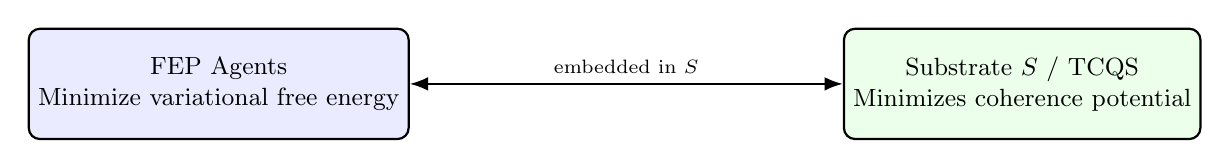
\begin{tikzpicture}[
    node distance=5.5cm,
    >=Latex,
    thick,
    box/.style={
        rectangle,
        rounded corners,
        draw,
        minimum width=4.1cm,
        minimum height=1.4cm,
        align=center,
        font=\small
    }
]

\node[box, fill=blue!8] (bio) {FEP Agents\\Minimize variational free energy};
\node[box, fill=green!8, right=of bio] (cos) {Substrate \(S\) / TCQS\\Minimizes coherence potential};

\draw[<->] (bio) -- node[above,font=\scriptsize] {embedded in \(S\)} (cos);

\end{tikzpicture}
\end{center}

\clearpage

% =============================================================
% SECTION III — ONE-PAGE EXECUTIVE SUMMARY
% =============================================================

\section*{SECTION III: One-Page Executive Summary}

\subsection*{Title}
\textbf{The Substrate \(S\) as a Unified Free-Energy Machine:  
From Cosmic Coherence to Biological Active Inference}

\subsection*{Problem}
Physics and neuroscience often treat the universe and the brain as separate domains. The TCQS framework proposes a time-crystalline Substrate \(S\) whose evolution follows a coherence gradient, while Friston's Free-Energy Principle (FEP) describes how biological agents minimize variational free energy to avoid surprise. How do these two perspectives connect?

\subsection*{Key Construction}

\begin{enumerate}
    \item Define a coherence scalar \(C(S)\) on the substrate and a coherence potential \(\Phi[C(S)]\).
    \item Model agents as coherent submanifolds \(S_A\subset\mcS\) with recognition density \(q(\vartheta|\mu)\) and substrate-conditioned priors \(p(\vartheta|S)\).
    \item Introduce the unified free-energy functional:
    \[
    \boxed{
    \mcF_{S}[S,q] = \Phi\!\big[C(S)\big]
    + \KL\big(q(\vartheta|\mu)\,\|\,p(\vartheta|S)\big).
    }
    \]
\end{enumerate}

\subsection*{Main Insight}

\begin{itemize}
    \item Minimizing \(\mcF_{S}\) with respect to \(S\) yields a \emph{coherence-driven free-energy gradient} for the entire universe (TCQS side).
    \item Minimizing \(\mcF_{S}\) with respect to \(q\) and actions reproduces \emph{active inference} and predictive coding at the level of agents (FEP side).
\end{itemize}

Thus:
\[
\text{FEP for agents} \;\subset\; \text{free-energy dynamics of the Substrate } S.
\]

\subsection*{One-Line Takeaway}

\textbf{Reality is a Substrate \(S\) drifting down a coherence-based free-energy gradient, and living systems are the regions where that gradient locally implements Friston-style active inference.}

\end{document}
